\documentclass[red]{beamer}
\setbeamertemplate{navigation symbols}{}
\usepackage[utf8x]{inputenc}
\usepackage{graphicx}
\usepackage{beamerthemeshadow}

\usetheme{CambridgeUS}
\setbeamercolor{itemize item}{fg=red} % all frames will have red bullets

\begin{document}
\title{Solving CAPTCHAs}
\author[MM, LM, SN, AS]{Mihai Maruseac, Lucian Mogoșanu, Sofia Neață, Adrian Șendroiu}
\date{March 2012}

\pgfdeclareimage{q}{img/q}

\maketitle

\begin{frame}{Admin}
  \begin{itemize}
    \item Team: UnCAPTCHA
      \begin{itemize}
        \item Mihai Maruseac
        \item Lucian Mogoșanu
        \item Sofia Neață
        \item Adrian Șendroiu
      \end{itemize}
    \item Repo: \url{https://github.com/mihaimaruseac/ssl}
  \end{itemize}
\end{frame}

\begin{frame}{Architecture - Overview}
	\begin{center}
	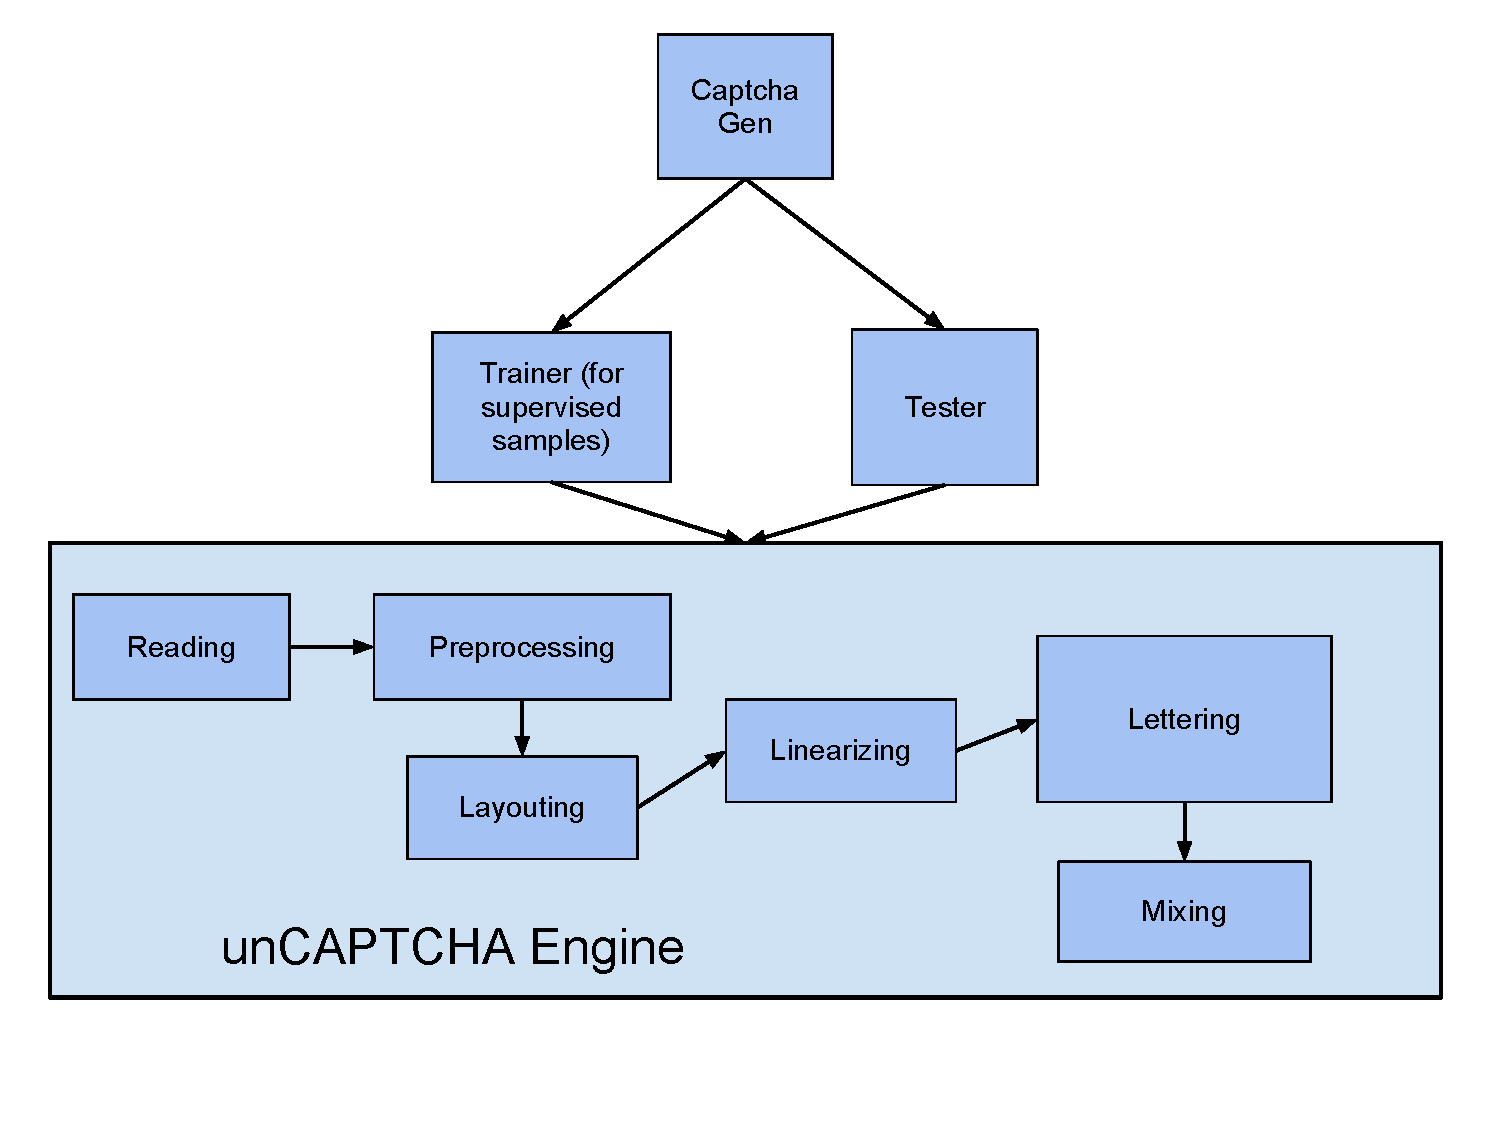
\includegraphics[width=0.85\textwidth]{img/unCAPTCHAarchitecturedraft.pdf}
	\end{center}
\end{frame}

\begin{frame}{Architecture - Overview}
  \begin{itemize}
  	\item Use Securimage to generate CAPTCHAs
	\item Feed them to a trainer and/or a tester
	\item Actual work done by the unCAPTCHA engine
	\begin{itemize}
		\item Pipelined architecture
		\item Easily extensible
	\end{itemize}
  \end{itemize}
\end{frame}

\begin{frame}{unCAPTCHA engine - Reading}
  \begin{itemize}
  	% TODO
	\item
  \end{itemize}
\end{frame}

\begin{frame}{unCAPTCHA engine - Preprocessing}
  \begin{itemize}
  	% TODO
	\item
  \end{itemize}
\end{frame}

\begin{frame}{unCAPTCHA engine - Layouting \& Linearizing}
  \begin{itemize}
  	% TODO
	\item
  \end{itemize}
\end{frame}

\begin{frame}{unCAPTCHA engine - Lettering \& Mixing}
  \begin{itemize}
  	% TODO
	\item
  \end{itemize}
\end{frame}

\begin{frame}{Thank you}
  \begin{center}
    \pgfuseimage{q}
  \end{center}
\end{frame}

\end{document}
